\bookchapter{NumPy: Fast Numbers}\label{ch:py8}

\section*{Explanation}
Joint angles of a walking gait, the pixels of a camera image, the weights of a neural network: all of them are \emph{tables of numbers}. Python lists can hold them, but a loop over a million list elements takes seconds. \textbf{NumPy} stores numbers in one compact block of memory and runs the loops in fast compiled code. It is also the basis of OpenCV (Chapter~\ref{ch:py10}), PyTorch and every other numerical library you will use, and its arrays are the vectors and matrices of the maths chapters. Install it in your virtual environment with \verb!pip install numpy! and import it by convention as \texttt{np}.

\section*{Arrays}
\begin{verbatim}
>>> import numpy as np
>>> a = np.array([1, 2, 3])
>>> a, a.dtype, a.shape
(array([1, 2, 3]), dtype('int64'), (3,))
>>> m = np.array([[1, 2, 3],
...               [4, 5, 6]])
>>> m.shape, m.ndim, m.size
((2, 3), 2, 6)
\end{verbatim}
An array has a \textbf{shape} (the length along each axis), a \textbf{dtype} (the number type, the same for all elements) and a number of dimensions. A shape of $(2,3)$ means $2$ rows and $3$ columns (Figure~\ref{fig:py8_axes}). A colour image is a $3$-dimensional array of shape \texttt{(height, width, 3)}.
\begin{center}
\begin{tikzpicture}[>={Stealth[length=2.5mm]}]
  \foreach \r in {0,1}{\foreach \c in {0,1,2}{
    \pgfmathtruncatemacro{\v}{\r*3+\c+1}
    \node[draw,thick,minimum size=0.9cm,fill=green!12,font=\footnotesize\ttfamily] at (\c,-\r) {\v};}}
  \node[font=\scriptsize,blue!60!black] at (0,0.7) {0}; \node[font=\scriptsize,blue!60!black] at (1,0.7) {1}; \node[font=\scriptsize,blue!60!black] at (2,0.7) {2};
  \node[font=\scriptsize,blue!60!black] at (-0.8,0) {0}; \node[font=\scriptsize,blue!60!black] at (-0.8,-1) {1};
  \draw[->,thick,red!70!black] (-1.3,0.5)--(-1.3,-1.5) node[midway,left,font=\footnotesize]{axis 0};
  \draw[->,thick,red!70!black] (-0.5,1.05)--(2.5,1.05) node[midway,above,font=\footnotesize]{axis 1};
  \node[font=\footnotesize\ttfamily,align=left,anchor=west] at (3.4,0.3) {m.shape = (2, 3)};
  \node[font=\footnotesize\ttfamily,align=left,anchor=west] at (3.4,-0.2) {m[1, 2] = 6};
  \node[font=\footnotesize\ttfamily,align=left,anchor=west] at (3.4,-0.7) {m[:, 1] = [2 5]};
  \node[font=\footnotesize\ttfamily,align=left,anchor=west] at (3.4,-1.2) {m.sum(axis=0) = [5 7 9]};
  \node[font=\footnotesize\ttfamily,align=left,anchor=west] at (3.4,-1.7) {m.sum(axis=1) = [6 15]};
\end{tikzpicture}
\captionof{figure}{A two-dimensional array. Axis $0$ runs down the rows, axis $1$ along the columns. \texttt{sum(axis=0)} collapses axis $0$ (one result per column).}\label{fig:py8_axes}
\end{center}
Ways to create arrays:
\begin{verbatim}
>>> np.zeros((2, 3)), np.ones(3), np.eye(2)       # eye = identity matrix
>>> np.arange(0, 1, 0.25)                         # like range, floats allowed
array([0.  , 0.25, 0.5 , 0.75])
>>> np.linspace(0, 1, 5)                          # 5 points including both ends
array([0.  , 0.25, 0.5 , 0.75, 1.  ])
>>> np.arange(6).reshape(2, 3)                    # same data, new shape
array([[0, 1, 2],
       [3, 4, 5]])
\end{verbatim}
\verb!reshape(3, -1)! lets NumPy calculate the missing length. \texttt{linspace} is better than \texttt{arange} for floats, since it avoids the rounding trouble of Chapter~\ref{ch:py1}.

\section*{Calculating with whole arrays}
Operations work on all elements at once, without a loop; this is called \textbf{vectorization}.
\begin{verbatim}
>>> a = np.array([1, 2, 3])
>>> a * 2, a + a, a ** 2          # element by element
(array([2, 4, 6]), array([2, 4, 6]), array([1, 4, 9]))
>>> a @ a                         # dot product (matrix product)
14
>>> np.sin(np.linspace(0, np.pi, 3))
array([0.0000000e+00, 1.0000000e+00, 1.2246468e-16])
\end{verbatim}
Note that \texttt{*} multiplies \emph{element by element}; the matrix product is \texttt{@}. A speed comparison shows why this matters (numbers vary with the computer):
\begin{verbatim}
big = np.random.rand(1_000_000)
s = 0.0
for v in big:             # Python loop:   about 0.16 s
    s += v * v
s2 = np.sum(big * big)    # NumPy:         about 0.005 s  (30 times faster)
\end{verbatim}
\begin{keyidea}[Think in arrays instead of loops]
If you write \texttt{for} over the elements of a NumPy array, stop and ask whether an array operation can do it. Typical speed-ups are $10$ to $100$ times. The loops still exist, but in compiled code.
\end{keyidea}

\section*{Indexing, slicing and masks}
\begin{verbatim}
>>> m = np.array([[1, 2, 3], [4, 5, 6]])
>>> m[1, 2], m[0], m[:, 1], m[:, ::2]
(6, array([1, 2, 3]), array([2, 5]), array([[1, 3],
                                            [4, 6]]))
\end{verbatim}
The syntax is \verb!m[rows, columns]! with the slices of Chapter~\ref{ch:py4}. A \textbf{boolean mask} selects elements by a condition:
\begin{verbatim}
>>> x = np.array([3., 1., 4., 1., 5., 9.])
>>> x > 2
array([ True, False,  True, False,  True,  True])
>>> x[x > 2]                       # only the elements where the mask is True
array([3., 4., 5., 9.])
>>> (x > 2).sum()                  # True counts as 1
4
>>> np.where(x > 2, 1, 0)          # choose between two values
array([1, 0, 1, 0, 1, 1])
>>> x[x > 8] = 0                   # assign through a mask
\end{verbatim}
Combine conditions with \verb!&! and \verb!|! (with parentheses), not with \texttt{and}/\texttt{or}: \verb!x[(x > 2) & (x < 6)]!.

\begin{keyidea}[Slices are views and not copies]
A slice of an array shares the memory with the original: changing the slice changes the array. This differs from lists, where slices are copies (Chapter~\ref{ch:py4}). Use \texttt{.copy()} when you need an independent array.
\end{keyidea}
\begin{verbatim}
>>> a = np.array([1, 2, 3])
>>> v = a[0:2]; v[0] = 7
>>> a                              # changed!
array([7, 2, 3])
\end{verbatim}

\section*{Statistics and reductions}
\begin{verbatim}
>>> x = np.array([3., 1., 4., 1., 5., 9.])
>>> x.mean(), x.std(), x.min(), x.argmax(), np.median(x)
(3.8333333333333335, 2.733536577809454, 1.0, 5, 3.5)
>>> m.sum(axis=0), m.sum(axis=1), m.mean(axis=1)
(array([5, 7, 9]), array([ 6, 15]), array([2., 5.]))
\end{verbatim}
\texttt{argmax} gives the \emph{position} of the maximum. Without \texttt{axis} the function uses all elements; with \texttt{axis=0} it collapses the rows (one result per column). The standard deviation here is the population version ($1/n$); use \texttt{ddof=1} for the sample version of Chapter~\ref{ch:stats}. Also useful: \texttt{np.clip(x, lo, hi)} (the clamp of Chapter~\ref{ch:py3} for whole arrays), \texttt{np.diff} (differences of neighbours, a discrete derivative), \texttt{np.cumsum}, \texttt{np.sort}, \texttt{np.argsort}.

\section*{Broadcasting}
What happens when you add arrays of different shapes? NumPy \emph{stretches} the smaller one if the shapes are compatible: compared from the right, each pair of lengths must be equal or one of them must be $1$.
\begin{verbatim}
>>> m = np.array([[1, 2, 3], [4, 5, 6]])     # shape (2, 3)
>>> m + np.array([10, 20, 30])               # (3,) is stretched over the rows
array([[11, 22, 33],
       [14, 25, 36]])
>>> np.array([[1], [2]]) + np.array([10, 20, 30])   # (2,1) + (3,) -> (2,3)
array([[11, 21, 31],
       [12, 22, 32]])
\end{verbatim}
\begin{center}
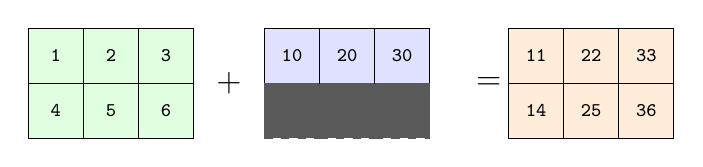
\begin{tikzpicture}[c/.style={draw,minimum size=0.7cm,font=\scriptsize\ttfamily,fill=green!12},s/.style={draw,dashed,minimum size=0.7cm,font=\scriptsize\ttfamily,fill=gray!15,gray!70!black}]
  \foreach \i in {0,1,2}{\node[c] at (\i*0.7,0.35) {\the\numexpr\i+1\relax}; \node[c] at (\i*0.7,-0.35) {\the\numexpr\i+4\relax};}
  \node[font=\large] at (2.2,0) {$+$};
  \foreach \i/\v in {0/10,1/20,2/30}{\node[c,fill=blue!12] at (3.0+\i*0.7,0.35) {\v}; \node[s] at (3.0+\i*0.7,-0.35) {\v};}
  \node[font=\large] at (5.5,0) {$=$};
  \foreach \i/\a/\b in {0/11/14,1/22/25,2/33/36}{\node[c,fill=orange!15] at (6.1+\i*0.7,0.35) {\a}; \node[c,fill=orange!15] at (6.1+\i*0.7,-0.35) {\b};}
\end{tikzpicture}
\captionof{figure}{Broadcasting: the row $[10,20,30]$ is virtually repeated for each row of the matrix (dashed). No copy is made.}\label{fig:py8_bc}
\end{center}
Broadcasting is how you subtract the mean from every column, scale an image, or compute all pairwise differences \texttt{x[:, None] - x[None, :]}. If shapes do not fit, NumPy raises \texttt{ValueError: operands could not be broadcast together}: print the shapes first.

\section*{Linear algebra}
\begin{verbatim}
>>> A = np.array([[2., 0.], [0., 3.]])
>>> v = np.array([1., 2.])
>>> A @ v, A.T                              # product, transpose
(array([2., 6.]), array([[2., 0.], [0., 3.]]))
>>> np.linalg.inv(A)                        # inverse
array([[0.5       , 0.        ],
       [0.        , 0.33333333]])
>>> np.linalg.solve(A, [2, 6])              # solves A x = b (better than inv)
array([1., 2.])
>>> np.linalg.det(A), np.linalg.norm([3, 4])
(6.0, 5.0)
\end{verbatim}
A rotation by the angle $\theta$ is the matrix $R=\begin{pmatrix}\cos\theta&-\sin\theta\\ \sin\theta&\cos\theta\end{pmatrix}$ (Block~3); applied to the point $(1,0)$ with $\theta=90^\circ$:
\begin{verbatim}
>>> th = np.pi / 2
>>> R = np.array([[np.cos(th), -np.sin(th)], [np.sin(th), np.cos(th)]])
>>> np.round(R @ np.array([1, 0]), 3)
array([0., 1.])
\end{verbatim}
Prefer \texttt{solve} to computing the inverse; it is faster and numerically safer. \texttt{np.linalg.eig} and \texttt{np.linalg.svd} give eigenvalues and the singular value decomposition.

\section*{Random numbers, files, types}
\begin{verbatim}
>>> rng = np.random.default_rng(0)           # seed: repeatable
>>> r = rng.normal(0, 1, 1000)               # 1000 samples of N(0, 1)
>>> round(r.mean(), 3), round(r.std(), 3)
(-0.048, 0.977)
>>> rng.integers(0, 10, 5)
array([8, 8, 8, 4, 4])
\end{verbatim}
The sample mean is not exactly $0$, as Chapter~\ref{ch:stats} explains. Save and load arrays:
\begin{verbatim}
np.savetxt("a.csv", m, delimiter=",")        # readable text
m2 = np.loadtxt("a.csv", delimiter=",")
np.save("a.npy", m); m3 = np.load("a.npy")   # exact, fast, binary
\end{verbatim}
\textbf{dtype} matters. Floats are \texttt{float64} by default; neural networks often use \texttt{float32} (half the memory). Images use \texttt{uint8} (integers $0\dots255$), which \emph{wrap around} on overflow:
\begin{verbatim}
>>> np.uint8(250) + np.uint8(10)
4                                            # (with a RuntimeWarning)
>>> img.astype(np.float32) / 255             # convert before calculating
\end{verbatim}
This is a classic bug when you brighten or subtract images; convert to a wider type first, calculate, and clip back with \texttt{np.clip(..., 0, 255).astype(np.uint8)}.

\begin{example}
\textbf{Smoothing and the derivative of a recorded joint angle.} The sensor delivers $100$ values per second. A moving average over $5$ values and the angular velocity:
\begin{verbatim}
t = np.linspace(0, 1, 101)                       # 101 points, 0.01 s apart
rng = np.random.default_rng(1)
angle = np.sin(2 * np.pi * t) + rng.normal(0, 0.05, t.size)   # noisy sine

kernel = np.ones(5) / 5
smooth = np.convolve(angle, kernel, mode="same")  # moving average
velocity = np.diff(smooth) / np.diff(t)           # rad/s, one value fewer
inner = velocity[3:-3]                            # skip the edge effects
print(velocity.shape, round(inner.max(), 1))      # (100,) 7.6
\end{verbatim}
The true derivative $2\pi\cos(2\pi t)$ has the maximum $2\pi\approx6.28$. Differentiating the \emph{raw} noisy angle gives values up to about $18$ rad/s, since noise of $0.05$ rad over $0.01$ s becomes several rad/s; the smoothed signal gives $7.6$, much closer. (The first and last points are skipped because \texttt{mode="same"} pads with zeros there.) Differentiation amplifies noise, which is why robots filter their sensor signals (Chapter~\ref{ch:py7} showed a filter class). We plot this in Chapter~\ref{ch:py9}.
\end{example}

\section*{Practice problems}
\begin{enumerate}[label=\textbf{\thechapter.\arabic*}]
  \item What are the shapes of \texttt{np.zeros((4, 3))}, \texttt{np.arange(12).reshape(3, 4)} and its transpose?
  \item Create the array of the squares of $1\dots10$ without a loop, and compute their sum and mean.
  \item With \texttt{x = np.array([3., 1., 4., 1., 5., 9.])}: write expressions for the elements larger than the mean, their number, and the index of the smallest element.
  \item Explain the difference between \texttt{a * b} and \texttt{a @ b} for two $3\times3$ matrices.
  \item What are the results of \verb!m.sum(axis=0)! and \verb!m.sum(axis=1)! for \verb!m = np.arange(6).reshape(2, 3)!?
  \item A $480\times640$ gray image \texttt{img} (type \texttt{uint8}) is to be brightened by $50$ levels without overflow. Write the code.
  \item Why does changing \texttt{b = a[:3]} also change \texttt{a} in NumPy, but not for a list? How do you avoid it?
  \item Which shape does the result have: \verb!np.ones((3, 1)) + np.ones((1, 4))!? Compute the matrix of all products $i\cdot j$ for $i,j=1\dots5$ with broadcasting.
  \item Solve $\begin{pmatrix}2&1\\1&3\end{pmatrix}\vec{x}=\begin{pmatrix}3\\5\end{pmatrix}$ with NumPy and check the result with \texttt{@}.
  \item[\textbf{\thechapter.10}$\star$] Generate $100\,000$ random numbers from a uniform distribution, compute the mean of $5$ of them at a time (reshape!), and check that the standard deviation of these means is close to $\sigma/\sqrt5$ (Chapter~\ref{ch:stats}). Compare with a Python loop in speed.
\end{enumerate}
